% =========================================================
% CONFIGURACION DEL DOCUMENTO
% =========================================================
\providecommand{\main}{..}
\documentclass[\main/Main.tex]{subfiles}

% =========================================================
% CONTENIDO
% =========================================================
\begin{document}
\chapter{Resultados}
\label{cha:04_resultados}
    % =====================================================
    % =====================================================
    \section{Modo de uso}
    \label{sec:04_modo_uso}
        Debido a las características de este trabajo de título se opta por presentar los resultados obtenidos a modo de manual de uso. En este sentido, y dado que la aplicación puede ser utilizada tanto en forma de \textit{\acrshort{api}} como de \textit{GUI}, se decide presentar desde estas dos perspectivas el proceso de configuración y ejecución de un experimento.

        El experimento a configurar estará conformado por dos tareas que se ejecutarán una sola vez, de forma secuencial y luego de presionar la tecla espacio: La primera tarea a configurar consistirá en un ejercicio de movimiento prosacádico bajo el paradigma de \textit{overlap}, lo que implica que el estímulo central se encontrará presente en todos los cuadros. De esta forma, se propone un cuadro inicial que contenga solo dicho estímulo identificado por una cruz blanca, con duración de $1.7[s]$. Luego, se presenta un cuadro que contenga además el punto objetivo identificado por un cuadro rojo, $16\degree$ a la derecha del estímulo inicial, durante $1.5[s]$. La segunda tarea consiste en la presentación de una imagen centrada para analizar patrones de búsqueda. En este caso el cuadro no debe ser temporizado: La tarea termina luego de que el usuario presione la tecla espacio. 

        La presentación de los estímulos se realizará utilizando el monitor secundario\footnote{Resolución de $1680x1050[px]$ y una pantalla con ancho efectivo de $47.5[cm]$.} que se encuentra ubicado a $53[cm]$ del paciente\footnote{La configuración del monitor debe ser realizada mediante el \textit{Monitor center} de \textit{psychoPy}. Al perfil correspondiente se le asigna el nombre ''my\_monitor'' por simplicidad.}. Además, se hará uso de un \textit{eye tracker} ''Eyetribe'' y los resultados obtenidos serán almacenados en el directorio \textref{''C:/SaccadeApp/events/''}.

        \newpage
        % =================================================
        \subsection{Usando la \textit{API}}
            \subsubsection{Configurar}
                En este proceso se utilizarán los siguientes módulos:
\begin{singlespace}\begin{python}
from saccadeapp.api import SaccadeDB
from saccadeapp.api import Configuration
from saccadeapp.api import Experiment, Test, Frame, Component
\end{python}\end{singlespace}

                El primer paso es contar con una base de datos disponible. Para crear una en el directorio donde se ejecutan los comandos se utiliza la siguiente instrucción: 
\begin{singlespace}\begin{python}
database = SaccadeDB()
\end{python}\end{singlespace}
        
                Luego, es posible crear el experimento propuesto:
\begin{singlespace}\begin{python}
# Experiment:
experiment = Experiment(db=database)
experiment.set_code(code=u"exp_0001")
experiment.set_info(name=u"Example Experiment", version=u"coded_1.0")
experiment.set_descripton(text=u"This experiment was created with code!")
experiment.set_space_start(status=True)
experiment.set_dialog(status=False)
experiment.set_random(status=False)
experiment.set_rest_conf(status=False)
\end{python}\end{singlespace}

                Las tareas que lo conforman:
\begin{singlespace}\begin{python}
### Test_1: Prosaccade ######
test1 = Test()
test1.set_name(u"Test 1")
# Test_1 - Frame_1: 
t1_fra1 = Frame()
t1_fra1.set_name(u"FP frame")
t1_fra1.set_color(u"black")
t1_fra1.set_as_task(False)
t1_fra1.set_time(1.7)
test1.add_item(t1_fra1)
# Test_1 - Frame_1 - FP
t1_fp = Component()
t1_fp.set_name(u"Fix Point")
t1_fp.set_shape(u"cross")
t1_fp.set_color(u"white")
t1_fp.set_position(0.0, 0.0)
t1_fra1.add_item(t1_fp)
# Test_1 - Frame_2:
t1_fra2 = t1_fra1.copy()
t1_fra2.set_name(u"TP frame")
t1_fra2.set_time(1.5)
test1.add_item(t1_fra2)
# Test_1 - Frame_2 - TP
t1_tp = Component()
t1_tp.set_name(u"Target Point")
t1_tp.set_shape(u"square")
t1_tp.set_color(u"red")
t1_tp.set_position(16.0, 0.0)
t1_fra2.add_item(t1_tp)
#Add test1 to experiment
experiment.add_item(test1)
#Add test1 to sequence
experiment.sequence_add(item_id=0, quantity=1)
\end{python}\end{singlespace}

\begin{singlespace}\begin{python}
### Test_2: Couple Image ####
test2 = Test()
test2.set_name(u"Test 2")
# Test_2 - Frame_1: 
t2_fra1 = Frame()
t2_fra1.set_name(u"Couple")
t2_fra1.set_color(u"black")
t2_fra1.set_as_task(True)
t2_fra1.set_keys_allowed(u"space")
t2_fra1.set_keys_correct(u"space")
test2.add_item(t2_fra1)
# Test_2 - Frame_1 - Image:
t2_img = Component()
t2_img.set_name(u"Couple Image")
t2_img.set_image(u"couple.png")
t2_fra1.add_item(t2_img)
#Add test2 to experiment
experiment.add_item(test2)
#Add test2 to sequence
experiment.sequence_add(item_id=1, quantity=1)
\end{python}\end{singlespace}

                Y el perfil de configuración requerido:
\begin{singlespace}\begin{python}
config_profile = Configuration(db=database)
config_profile.set_name(name=u"Test Profile (code)")
config_profile.set_events_path(path=u"C:/SaccadeApp/events/")
config_profile.set_tracker(tracker=u"eyetribe")
config_profile.set_monitor(monitor=u"my_Monitor")
config_profile.set_screen(screen=1)
\end{python}\end{singlespace}
    
                Finalmente se almacena en la base de datos tanto el experimento como el perfil de configuración:
\begin{singlespace}\begin{python}
experiment.save()
config_profile.save()
\end{python}\end{singlespace}

            \subsubsection{Ejecutar}
                Para ejecutar el experimento que acaba de ser configurado y almacenado en la base de datos según las condiciones propuestas basta utilizar los siguientes comandos:
\begin{singlespace}\begin{python}
from saccadeapp.app import ExperimentHandler

handler = ExperimentHandler()
handler.prepare(exp_code=u"exp_0001", conf_name=u"Test Profile (code)")
handler.execute(frame_save=True)
\end{python}\end{singlespace}

        \newpage
        % =================================================
        \subsection{Usando la \textit{GUI}}
            \subsubsection{Configurar}
                El primer paso consiste en añadir un perfil de configuración. Para esto es necesario ir a la pestaña \textref{Configuration} en la ventana principal.
                \begin{figure}[H]
                    \centering
                    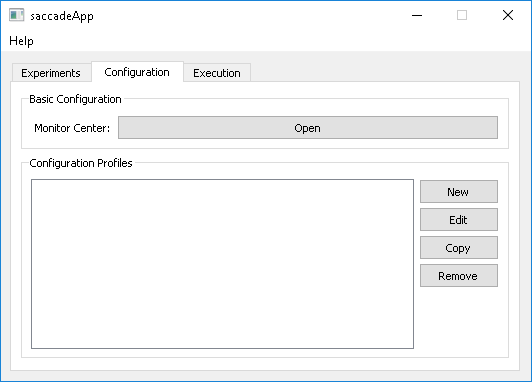
\includegraphics[width=0.52\textwidth]{cap_04_gui_00}
                    \caption{Pestaña de configuración.}
                    \label{fig:04_gui_conf00}
                \end{figure}

                Se crea un nuevo perfil donde se ingresan las configuraciones propuestas para el ejemplo, como se muestra a continuación:
                \begin{figure}[H]
                    \centering
                    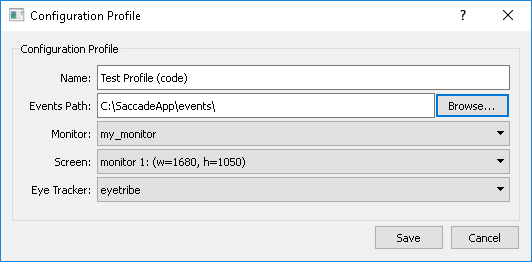
\includegraphics[width=0.52\textwidth]{cap_04_gui_01}
                    \caption{Perfil de configuración propuesto.}
                    \label{fig:04_gui_conf01}
                \end{figure}

                Luego, se finaliza la operación presionando el botón \textref{Save}.

                \newpage
                El segundo paso consiste en añadir un nuevo experimento. Para esto es necesario ir a la pestaña \textref{Experiment} en la ventana principal.
                \begin{figure}[H]
                    \centering
                    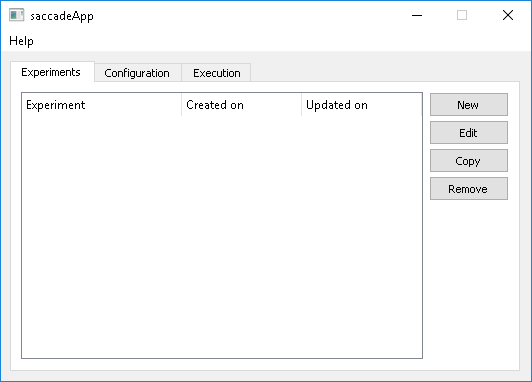
\includegraphics[width=0.52\textwidth]{cap_04_gui_02}
                    \caption{Pestaña de experimentos.}
                    \label{fig:04_gui_exp01}
                \end{figure} 

                Se crea un nuevo experimento donde se ingresan las configuraciones propuestas y se añade la primera tarea.
                \begin{figure}[H]
                    \centering
                    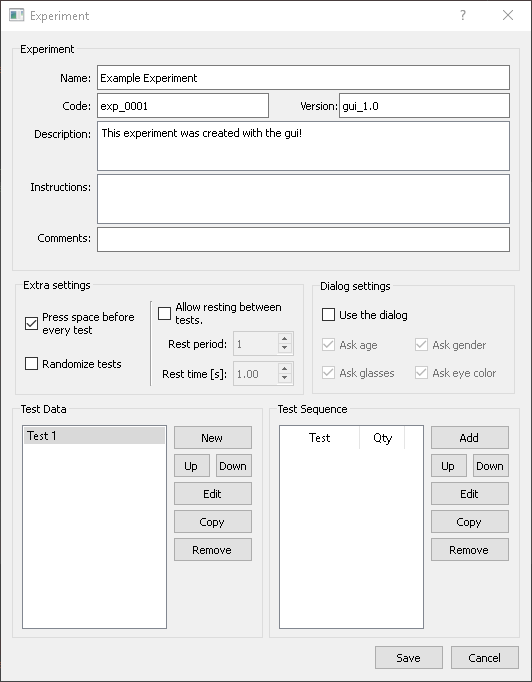
\includegraphics[width=0.43\textwidth]{cap_04_gui_03}
                    \caption{Experimento propuesto con la primera tarea configurada.}
                    \label{fig:04_gui_exp02}
                \end{figure} 

                \newpage
                \vspace{-6mm}
                Dicha tarea se compone de dos cuadros: 
                \begin{figure}[H]
                    \centering
                    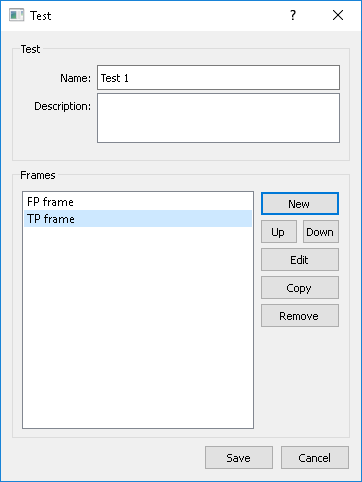
\includegraphics[width=0.40\textwidth]{cap_04_gui_04}
                    \caption{Ventana de configuración de la primera tarea.}
                    \label{fig:04_gui_exp03}
                \end{figure} 

                \vspace{-6mm}
                Que se encuentran configurados de la forma:
                \begin{figure}[H]
                    \centering
                    \subfloat[Primer cuadro.]{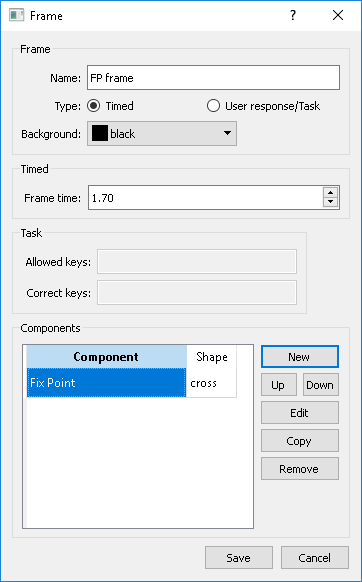
\includegraphics[width=0.40\textwidth]{cap_04_gui_05}} \hspace{5mm}
                    \subfloat[Segundo cuadro.]{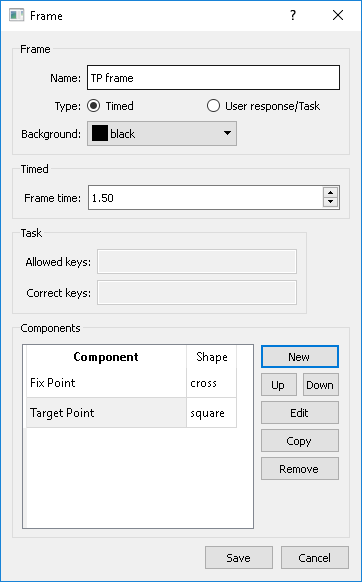
\includegraphics[width=0.40\textwidth]{cap_04_gui_06}}
                    \caption{Configuración de los cuadros pertenecientes a la primera tarea.}
                    \label{fig:04_gui_exp04}
                \end{figure} 

                \newpage
                \vspace{-6mm}
                Y donde los componentes que las conforman corresponden a: 
                \begin{figure}[H]
                    \centering
                    \subfloat[Punto de fijación.]{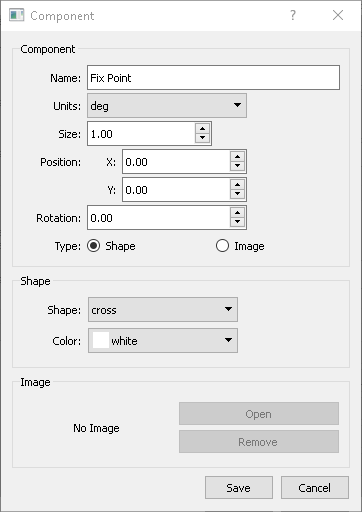
\includegraphics[width=0.40\textwidth]{cap_04_gui_07}} \hspace{5mm}
                    \subfloat[Punto objetivo.]{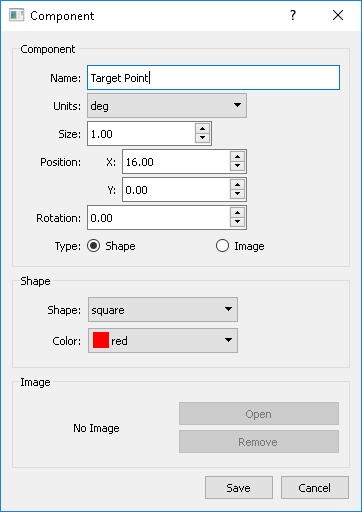
\includegraphics[width=0.40\textwidth]{cap_04_gui_08}}
                    \caption{Componentes utilizados en la configuración de la primera tarea.}
                    \label{fig:04_gui_exp05}
                \end{figure} 

                \vspace{-6mm}
                Para agregar la tarea a la secuencia de ejecución se utiliza el botón \textref{Add} de la lista de secuencias, lo que despliega la siguiente ventana: 
                \begin{figure}[H]
                    \centering
                    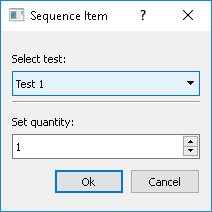
\includegraphics[width=0.4\textwidth]{cap_04_gui_09}
                    \caption{Agregando la primera tarea a la secuencia de ejecución.}
                    \label{fig:04_gui_exp06}
                \end{figure} 

                \newpage
                \vspace{-6mm}
                Luego de añadir ese elemento se obtiene el siguiente resultado:
                \begin{figure}[H]
                    \centering
                    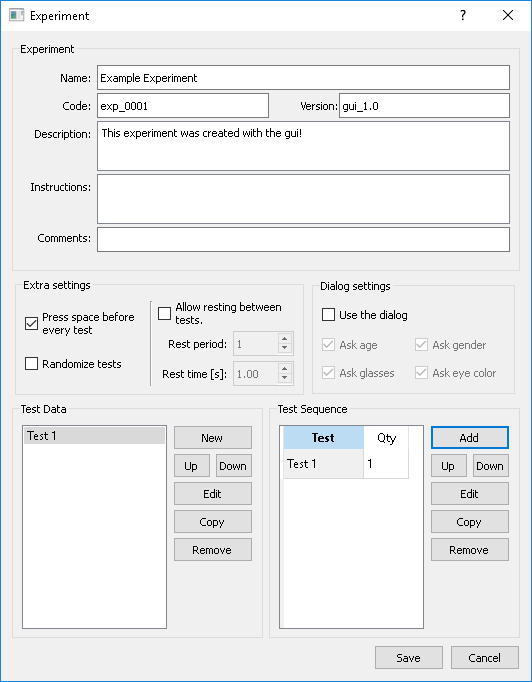
\includegraphics[width=0.43\textwidth]{cap_04_gui_10}
                    \caption{Experimento propuesto con la primera tarea configurada y en la secuencia de ejecución.}
                    \label{fig:04_gui_exp07}
                \end{figure} 

                \vspace{-6mm}
                De forma posterior se añade la segunda tarea, que solo se compone de un cuadro.
                \begin{figure}[H]
                    \centering
                    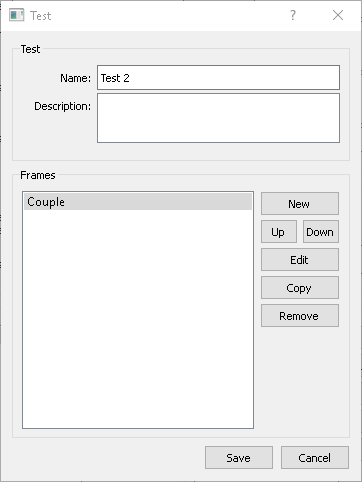
\includegraphics[width=0.40\textwidth]{cap_04_gui_11}
                    \caption{Ventana de configuración de la segunda tarea.}
                    \label{fig:04_gui_exp08}
                \end{figure} 

                \newpage
                \vspace{-6mm}
                Que presenta las siguientes configuraciones: 
                \begin{figure}[H]
                    \centering
                    \subfloat[Cuadro que contiene la imagen.]{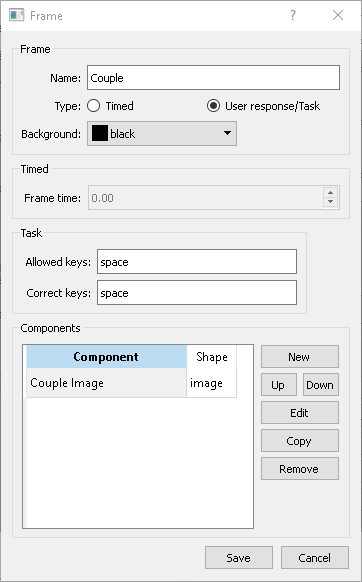
\includegraphics[width=0.40\textwidth]{cap_04_gui_12}} \hspace{5mm}
                    \subfloat[Imagen de la pareja.]{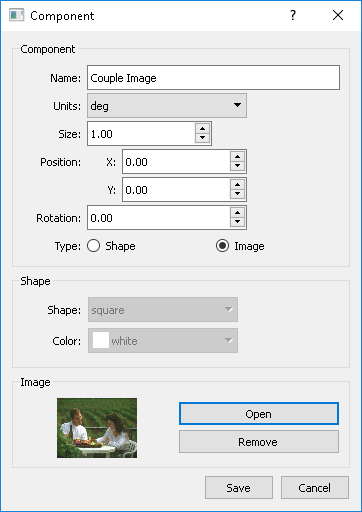
\includegraphics[width=0.40\textwidth]{cap_04_gui_13}}
                    \caption{Configuraciones de la segunda tarea.}
                    \label{fig:04_gui_exp09}
                \end{figure} 

                \vspace{-6mm} 
                Al añadir esta tarea a la secuencia de ejecución, el experimento queda de la forma: 
                \begin{figure}[H]
                    \centering
                    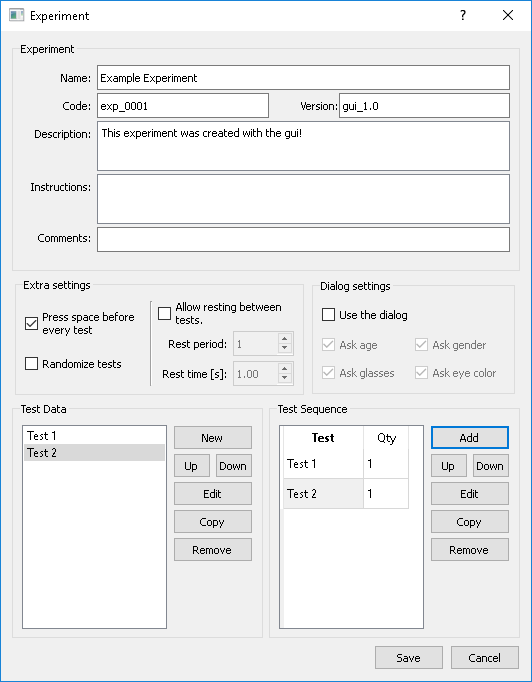
\includegraphics[width=0.43\textwidth]{cap_04_gui_14}
                    \caption{Experimento propuesto con configuración completa.}
                    \label{fig:04_gui_exp10}
                \end{figure} 

                \newpage
                Luego, se finaliza la operación presionando el botón \textref{Save}.

                Con estas configuraciones ya es posible ejecutar un experimento. Las pestañas de configuración, luego de añadir estos elementos quedan de la siguiente forma:
                \begin{figure}[H]
                    \centering
                    \subfloat[Pestaña de experimentos.]{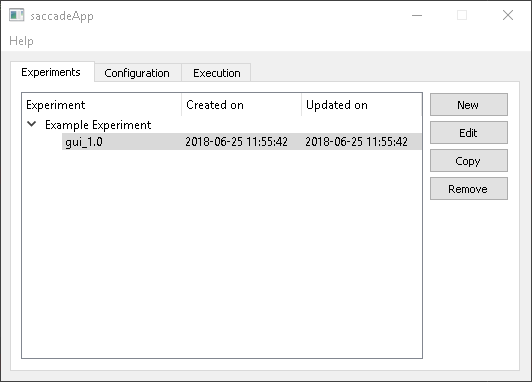
\includegraphics[width=0.45\textwidth]{cap_04_gui_15}} \hspace{5mm}
                    \subfloat[Pestaña de configuración.]{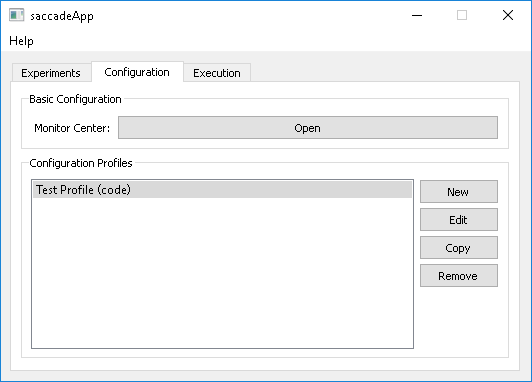
\includegraphics[width=0.45\textwidth]{cap_04_gui_16}}
                    \caption{Resultado obtenido.}
                    \label{fig:04_gui_final_01}
                \end{figure} 

            \subsubsection{Ejecutar}
                Para ejecutar el experimento es necesario ir a la pestaña \textref{Execution} en la ventana principal y seleccionar los elementos de interés de las listas desplegables:
                \begin{figure}[H]
                    \centering
                    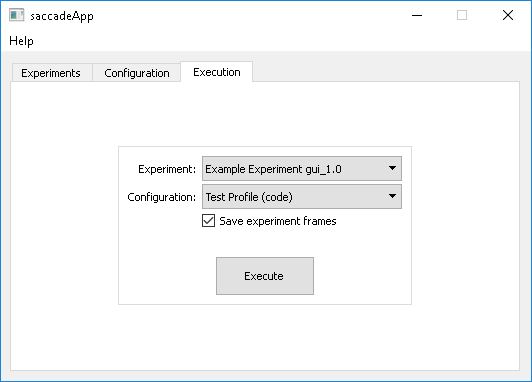
\includegraphics[width=0.52\textwidth]{cap_04_gui_17}
                    \caption{Aplicación lista para ejecutar \textit{script}.}
                    \label{fig:04_gui_final_02}
                \end{figure} 

                Finalmente se debe presionar el botón \textref{Execute}.

    \newpage
    % =====================================================
    % =====================================================
    \section{Comprobación de funcionamiento.}
    \label{sec:04_funcionamiento}
        Con el fin de comprobar el funcionamiento de la aplicación y asegurar el correcto registro de los datos se creó un experimento cuya única tarea consistía en realizar un ejercicio de inspección visual sobre la imagen presentada en la figura \ref{fig:04_frame_result} (a). 
        \begin{figure}[H]
            \centering
            \subfloat[Imagen original.]{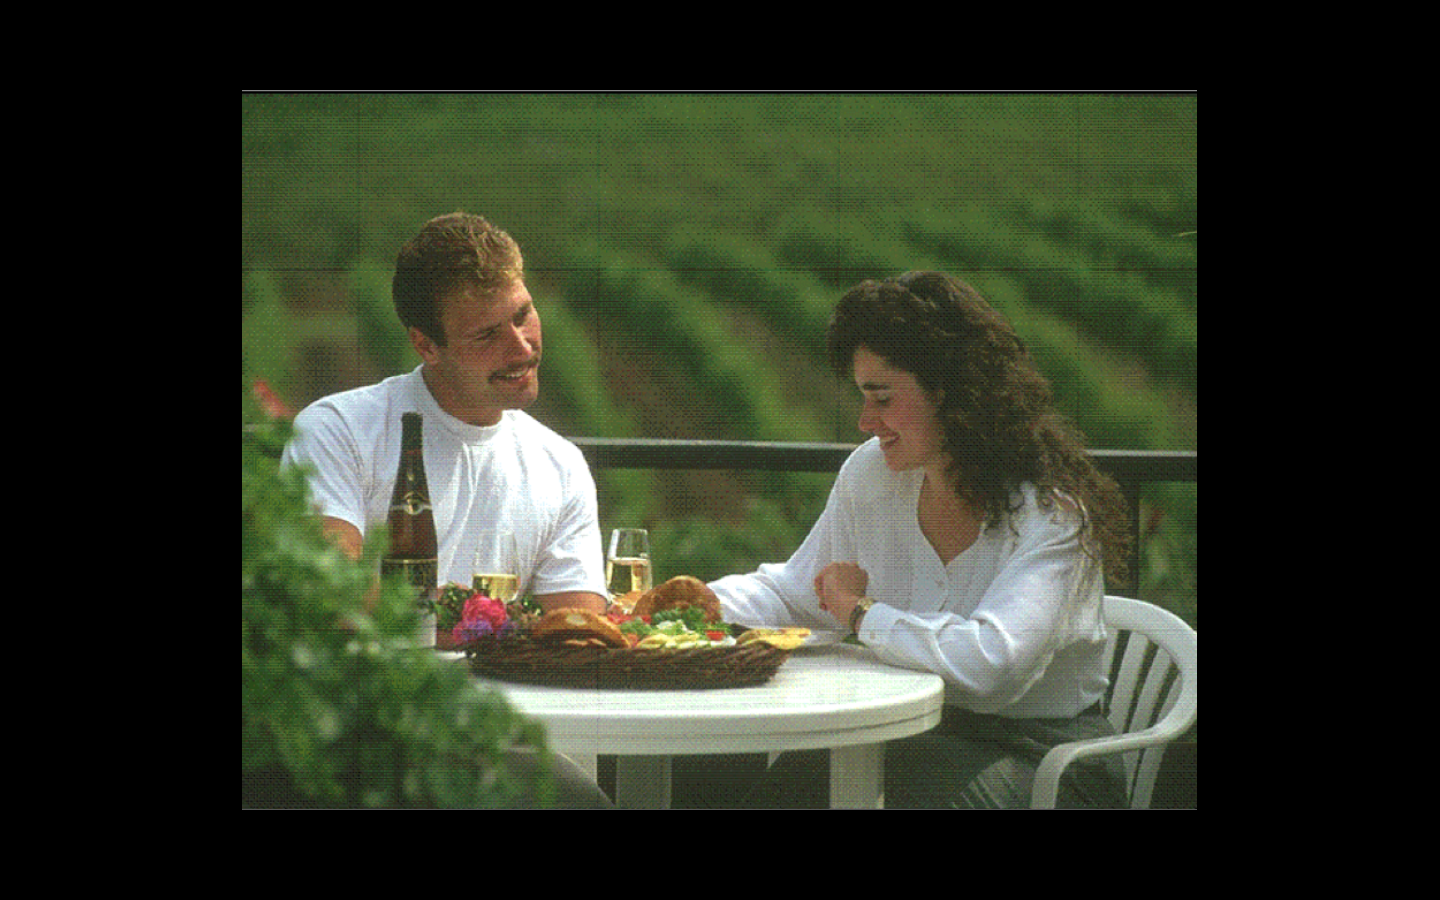
\includegraphics[width=0.45\textwidth]{cap_04_resultado_orig}}\\
            \subfloat[Movimiento ocular esperado.]{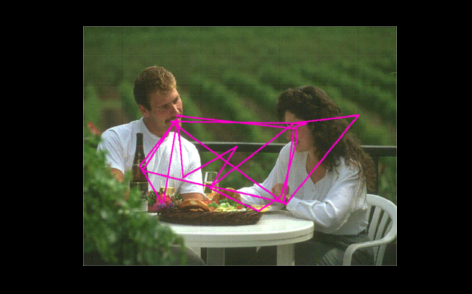
\includegraphics[width=0.45\textwidth]{cap_04_resultado_espe}}\hspace{5mm}
            \subfloat[Movimiento ocular registrado.]{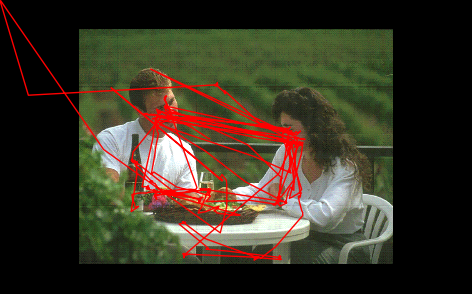
\includegraphics[width=0.45\textwidth]{cap_04_resultado_obte}}
            \caption{Datos registrados.}
            \label{fig:04_frame_result}
        \end{figure}

        Los datos registrados desde el \textit{eye tracker} en este experimento (\ref{fig:04_frame_result} (c)) muestran ser similares a los esperados (\ref{fig:04_frame_result} (b)), e indican que el movimiento ocular se realiza principalmente entre los rostros de la pareja y las proyecciones de hacia donde se encuentran dirigidas sus miradas. 

        Al consultar los registros de los puntos anómalos presentes principalmente en la esquina superior izquierda y que parecieran no corresponder al patrón de observación, se determina que se encuentran relacionados a los momentos en que el usuario cierra los ojos y no es posible realizar estimaciones de la posición ocular.    

\end{document}
